\documentclass[a4paper]{article}

\usepackage[portuguese]{babel}
\usepackage{graphicx}
\usepackage[a4paper, margin=2.5cm]{geometry}
\usepackage{indentfirst}
\usepackage{listings}
\usepackage{xcolor}
\usepackage{float}
\usepackage[utf8]{inputenc}
\usepackage[hidelinks]{hyperref}
\usepackage{booktabs}
\usepackage{array}
\usepackage{longtable}
\usepackage{multirow}
\usepackage{enumitem}
\usepackage{tikz}
\usepackage{pgfplots}
\usepackage{amssymb}
\pgfplotsset{compat=1.18}

\lstset{
    language=Java,
    basicstyle=\ttfamily\small,
    keywordstyle=\color{blue},
    stringstyle=\color{red},
    commentstyle=\color{gray},
    breaklines=true,
    frame=single,
    numbers=left,
    numberstyle=\tiny\color{gray},
    numbersep=5pt
}

\begin{document}

\begin{titlepage}
    \centering
    \begin{figure}[h]
        \centering
        
\includegraphics[width=0.3\textwidth]{images/eeum.png}
        \label{fig:logo}
    \end{figure}
    \vspace{2cm}

    {\huge\bfseries Trabalho Prático POO\par}
    \vspace{2cm}

    {\large
    {\bfseries Grupo G036}
 
    \vspace{1cm}
 
    \begin{tabular}{>{\centering\arraybackslash}m{4cm}>{\centering\arraybackslash}m{2cm}>{\centering\arraybackslash}m{4cm}}
        Gabriel Faria & a111532 & 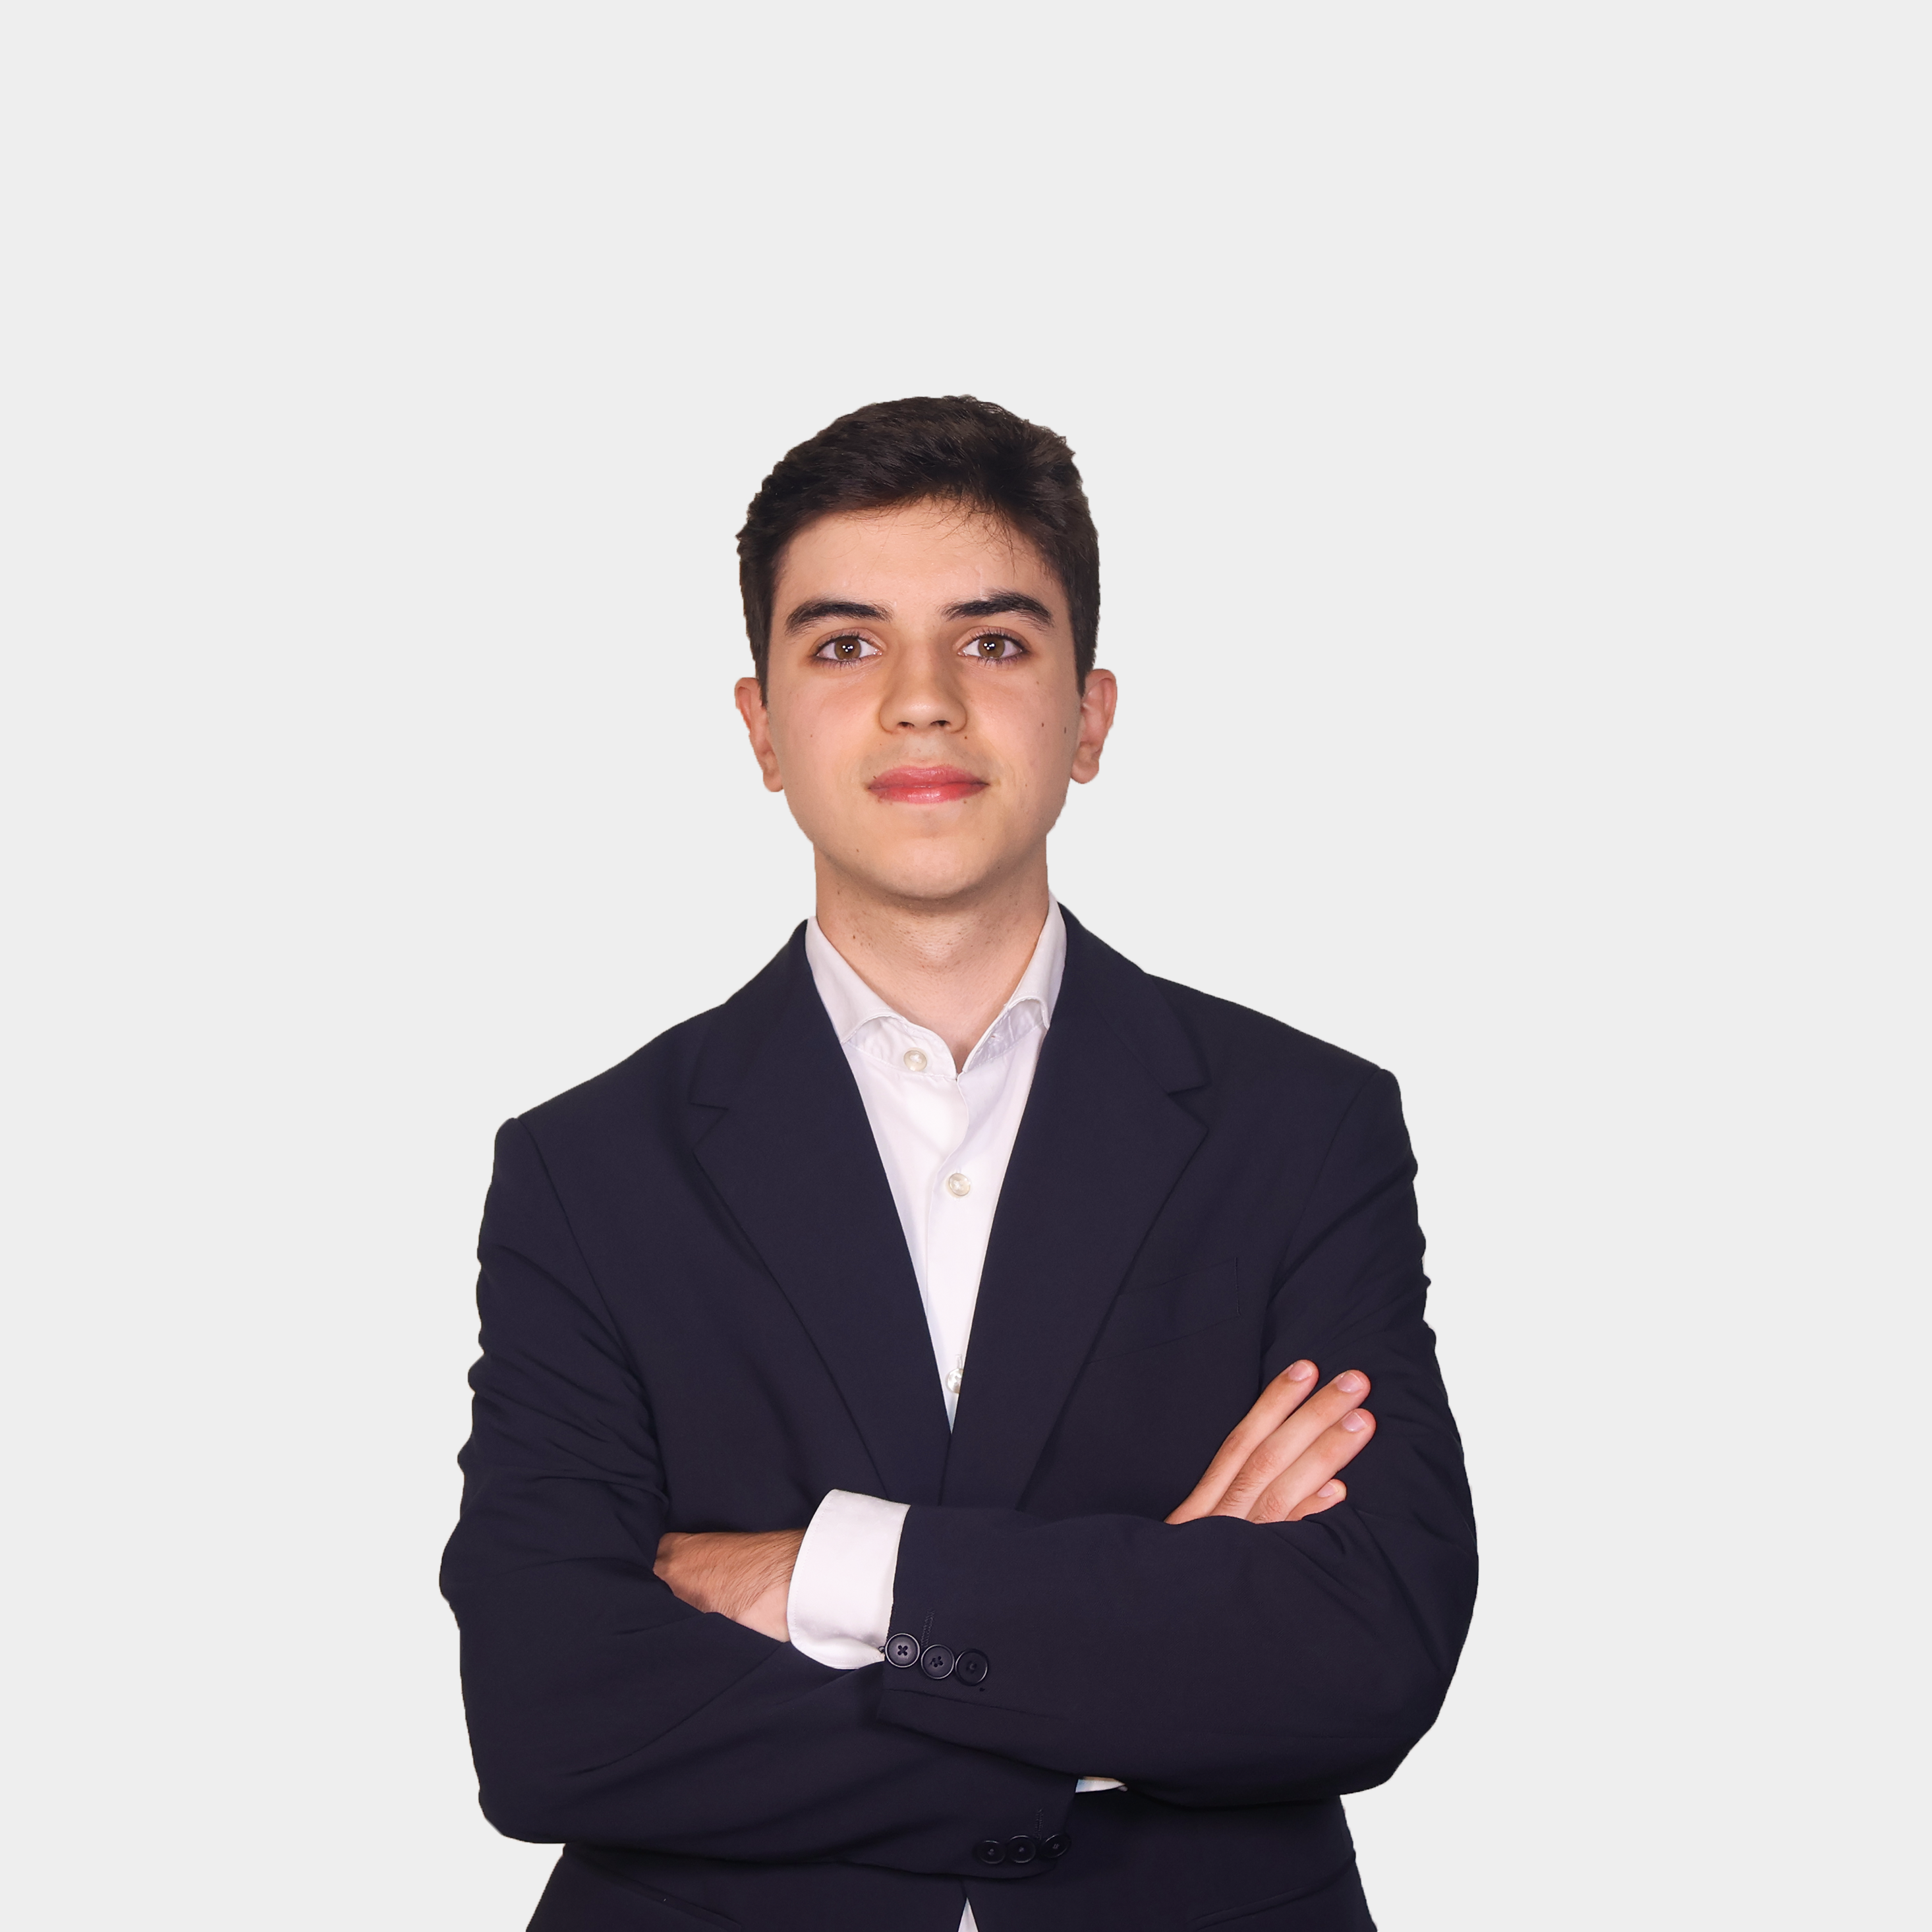
\includegraphics[width=3cm, height=3.5cm, keepaspectratio]{images/gabrielfaria.png} \\[1cm]
        Ricardo Rodrigues & a111225 & 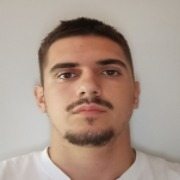
\includegraphics[width=3cm, height=3.5cm, keepaspectratio]{images/ricardorodrigues.jpeg} \\[1cm]
        Rui Gomes & a111273 & 
\includegraphics[width=3cm, height=3.5cm, keepaspectratio]{images/ruigomes.jpeg} \\[1cm]
    \end{tabular}
 
    \vspace{1.5cm}
 
    Licenciatura em Engenharia Informática \\
    Universidade do Minho \\
    2025/2026
    \par}


\end{titlepage}

\tableofcontents
\newpage

\section{Introdução}

O \textbf{DomusControl} é uma aplicação de automação doméstica desenvolvida no âmbito da unidade curricular de Programação Orientada aos Objectos (POO), inspirada em sistemas como o \textit{Home Assistant}. O sistema permite gerir casas, divisões, dispositivos e mecanismos de automatização através de uma interface textual por menus.

O desenvolvimento seguiu rigorosamente os princípios da programação orientada aos objectos, como encapsulamento, herança, polimorfismo e abstração. O relatório está organizado da seguinte forma: a Secção~2 descreve a arquitetura de classes do sistema, a Secção~3 apresenta as principais decisões de design, a Secção~4 descreve a aplicação e as suas funcionalidades, a Secção~5 apresenta os testes automatizados realizados e a Secção~6 conclui o relatório.

\section{Arquitetura do Sistema}

A arquitetura do DomusControl segue um modelo orientado aos objectos, organizado em packages bem definidos. O sistema é composto por dispositivos domésticos de vários tipos, agrupados em divisões, que por sua vez pertencem a casas. Os mecanismos de automação - automações, escalonamentos e cenários - operam sobre estes dispositivos. O DomusControl coordena todas as operações, delegando em serviços especializados.

\subsection{Organização em Packages}

O projeto está organizado nos seguintes packages principais:

\begin{itemize}
    \item \texttt{org.domuscontrol} - Classe \texttt{Utilizador} e ponto de entrada (\texttt{Main})
    \item \texttt{org.domuscontrol.casa} - Classes \texttt{Casa} e \texttt{Divisao}
    \item \texttt{org.domuscontrol.dispositivos} - Hierarquia de dispositivos
    \item \texttt{org.domuscontrol.mecanismos} - Automações, escalonamentos, cenários e ações
    \item \texttt{org.domuscontrol.model} - \texttt{DomusControl} e serviços
    \item \texttt{org.domuscontrol.model.services} - Serviços especializados do modelo
    \item \texttt{org.domuscontrol.exceptions} - Exceções específicas do domínio
    \item \texttt{org.domuscontrol.ui} - Interface textual (\texttt{TextUI}, \texttt{Menu})
    \item \texttt{org.domuscontrol.ui.menus} - Sub-menus por entidade
\end{itemize}

\subsection{Dispositivos}

A hierarquia de dispositivos é baseada em herança a partir de uma classe abstrata \texttt{Dispositivo}. Esta arquitetura permite adicionar novos tipos de dispositivos sem alterar o código existente.

\begin{center}
\begin{tabular}{ll}
    \toprule
    \textbf{Classe} & \textbf{Atributos específicos} \\
    \midrule
    \texttt{Dispositivo} (base) & \texttt{id}, \texttt{marca}, \texttt{modelo}, \texttt{consumoPorHora}, \texttt{estado} \\
    \texttt{ArCondicionado} & \texttt{temperatura}, \texttt{tempMin}, \texttt{tempMax} \\
    \texttt{Aspirador} & \texttt{intensidade}, \texttt{intensidadeMax} \\
    \texttt{CamaraVigilancia} & \texttt{visaoNoturna}, \texttt{visaoInfraVermelho} \\
    \texttt{Coluna} & \texttt{volume} \\
    \texttt{Forno} & \texttt{temperatura}, \texttt{tempMax} \\
    \texttt{Lampada} & \texttt{intensidade}, \texttt{intensidadeMax} \\
    \texttt{Persiana} & \texttt{percentagemAbertura} \\
    \texttt{Portao} & \texttt{percentagemAbertura} \\
    \texttt{Televisao} & \texttt{volume}, \texttt{brilho} \\
    \bottomrule
\end{tabular}
\end{center}

O \texttt{Dispositivo} tem um contador estático \texttt{proxId} para garantir identificadores únicos e auto-incrementados.

\subsection{Casa e Divisão}

A \texttt{Casa} agrega \texttt{Divisao} (num \texttt{Map<Integer, Divisao>}) e cada \texttt{Divisao} agrega \texttt{Dispositivo}. A \texttt{Casa} também agrega diretamente listas de mecanismos: \texttt{List<Automacao>}, \texttt{List<Escalonamento>} e \texttt{List<Cenario>}.

A relação é de \textbf{agregação}: os dispositivos existem independentemente das divisões e as casas existem independentemente dos utilizadores. Não são usados clones ao guardar nas coleções internas.

\subsection{Mecanismos}

Todos os mecanismos derivam da classe \texttt{Mecanismo}, que contém:

\begin{itemize}
    \item \texttt{identificador} (auto-gerado), \texttt{nome}, \texttt{descricao}
    \item \texttt{List<AcaoDispositivo> acoes} - lista de ações a executar
    \item Método \texttt{executarAcoes(Casa)} que itera e executa todas as ações
\end{itemize}

As ações implementam a interface \texttt{AcaoDispositivo}:

\begin{center}
\begin{tabular}{ll}
    \toprule
    \textbf{Ação} & \textbf{Efeito} \\
    \midrule
    \texttt{AcaoLigar} & Liga um dispositivo numa divisão \\
    \texttt{AcaoDesligar} & Desliga um dispositivo \\
    \texttt{AcaoMudarTemperatura} & Altera a temperatura do A/C ou Forno \\
    \texttt{AcaoMudarIntensidadeLampada} & Altera a intensidade de uma lâmpada \\
    \bottomrule
\end{tabular}
\end{center}

As condições de automação implementam a interface \texttt{CondicaoAutomacao}:

\begin{center}
\begin{tabular}{ll}
    \toprule
    \textbf{Condição} & \textbf{Avaliação} \\
    \midrule
    \texttt{CondicaoDispositivoLigado} & Verdade se o dispositivo estiver ligado \\
    \texttt{CondicaoDispositivoDesligado} & Verdade se o dispositivo estiver desligado \\
    \texttt{CondicaoTemperaturaMaiorQue} & Verdade se a temp.\ do A/C exceder o limite \\
    \texttt{CondicaoConsumoMaiorQue} & Verdade se o consumo total exceder o limite \\
    \bottomrule
\end{tabular}
\end{center}

\textbf{Automação}: verifica a condição em cada avaliação e executa as ações quando a condição passa de falsa para verdadeira (evitando execuções repetidas). O flag \texttt{condicaoAtiva} gere este estado.

\textbf{Escalonamento}: dispara as ações numa hora específica (em minutos desde meia-noite). Pode ser diário ou por dias específicos da semana. O campo \texttt{ultimoTempoDisparado} evita múltiplos disparos no mesmo minuto.

\textbf{Cenário}: tem duas listas de ações - \texttt{acoes} (ativação) e \texttt{acoesDesativacao}. O flag \texttt{ativo} controla o estado. Os métodos \texttt{ativar()}, \texttt{desativar()} e \texttt{alternar()} gerem as transições.

\subsection{Utilizador e Histórico de Interações}

O \texttt{Utilizador} mantém duas coleções de casas:

\begin{itemize}
    \item \texttt{Map<Integer, Casa> casas} - casas de acesso normal
    \item \texttt{Map<Integer, Casa> casasAdmin} - casas com permissão de administrador
\end{itemize}

Regista também um histórico de \texttt{List<Interacao>}, onde cada \texttt{Interacao} guarda momento, casa, divisão, dispositivo e tipo de ação. Este histórico alimenta o motor de sugestões.

\subsection{Motor de Sugestões}

O método \texttt{gerarSugestoes()} no \texttt{Utilizador} analisa o histórico de interações e agrupa-as por \textit{(hora, dispositivo, ação)}. Quando um padrão se repete pelo menos 3 vezes, gera um \texttt{Escalonamento} sugerido. O utilizador pode aceitar a sugestão e ela é adicionada a uma casa da sua escolha.

\subsection{Modelo e Serviços}

A classe \texttt{DomusControl} funciona como \textbf{fachada} do sistema. Mantém os mapas de utilizadores e casas e delega operações especializadas em serviços:

\begin{center}
\begin{tabular}{ll}
    \toprule
    \textbf{Serviço} & \textbf{Responsabilidade} \\
    \midrule
    \texttt{UtilizadoresECasasModel} & Associar/remover utilizadores de casas, permissões \\
    \texttt{DispositivoModel} & Adicionar/remover/operar dispositivos \\
    \texttt{DivisoesModel} & Gestão de divisões \\
    \texttt{AutomacoesModel} & Listagem de condições disponíveis \\
    \texttt{EscalonamentosModel} & Serviço de escalonamentos \\
    \texttt{CenariosModel} & Serviço de cenários \\
    \texttt{FicheirosModel} & Guardar/carregar estado em ficheiro binário \\
    \texttt{TopsModel} & Estatísticas e rankings \\
    \bottomrule
\end{tabular}
\end{center}

\subsection{Padrão Model-View-Controller}

A arquitetura do DomusControl segue o padrão \textbf{Model-View-Controller (MVC)}, separando claramente as responsabilidades entre a lógica de negócio, a interface com o utilizador e o controlo do fluxo da aplicação. A figura seguinte ilustra esta organização.

\begin{figure}[H]
    \centering
    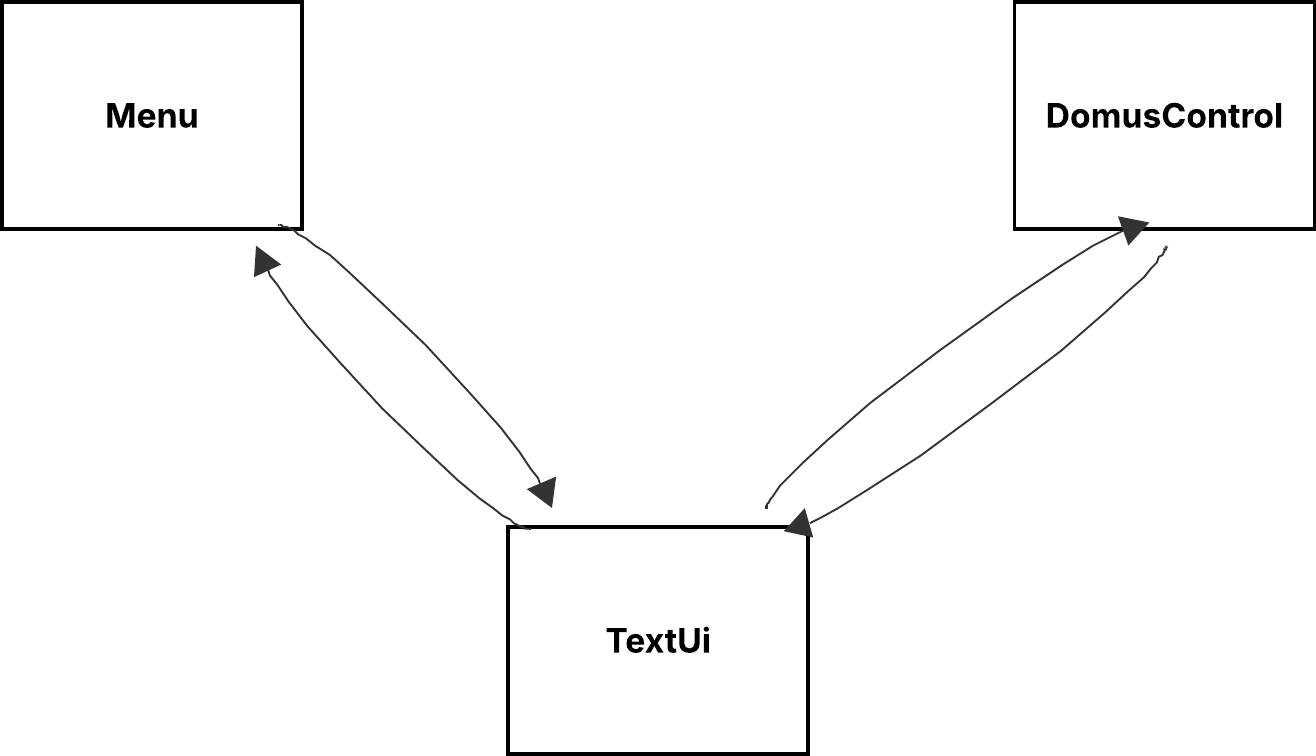
\includegraphics[width=1\textwidth]{images/mvc.png}
    \caption{Arquitetura MVC do DomusControl.}
    \label{fig:mvc}
\end{figure}

\subsection{Diagrama de Classes}

O diagrama de classes seguinte apresenta as principais classes do sistema e as relações entre elas.

\begin{figure}[H]
    \centering
    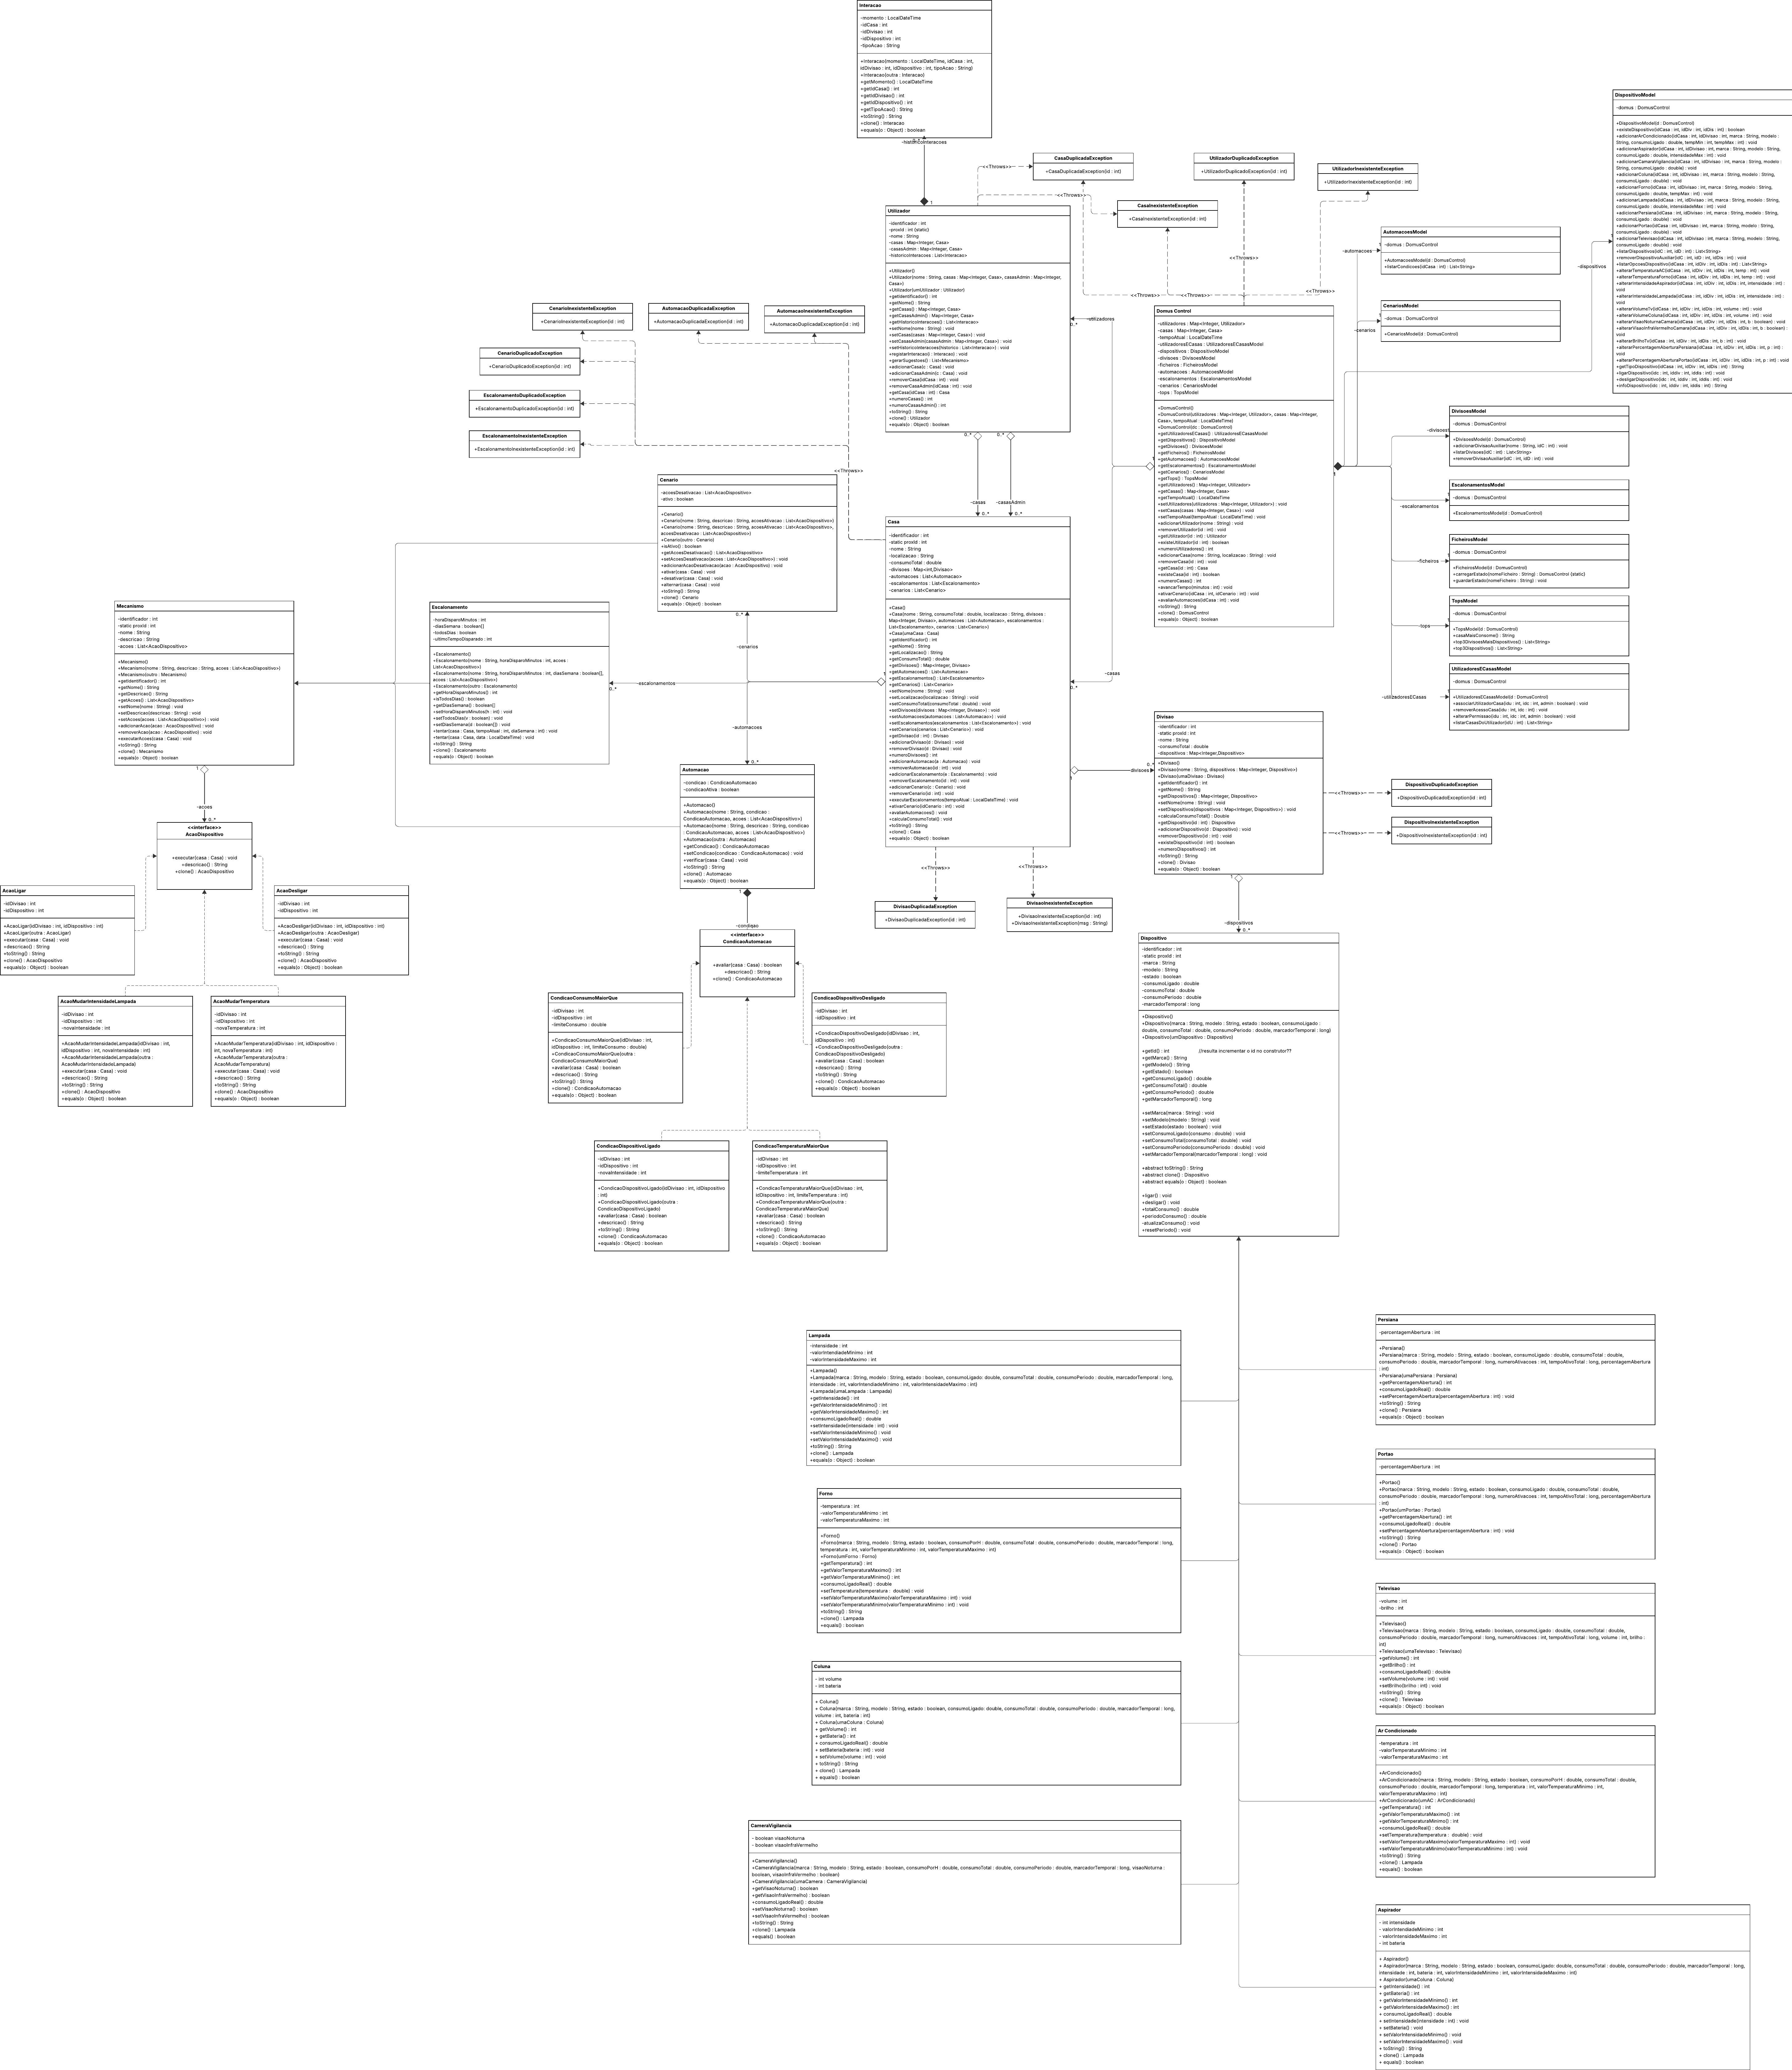
\includegraphics[width=\textwidth]{images/DiagramaClasses.png}
    \caption{Diagrama de classes do DomusControl.}
    \label{fig:diagrama}
\end{figure}

\section{Decisões de Design}

\subsection{Agregação vs.\ Composição}

Uma das principais decisões foi usar \textbf{agregação} em vez de composição. Os mecanismos e as ações são referenciados por referência nas coleções - não são clonados ao ser adicionados. Esta abordagem garante que uma alteração ao objeto original se reflete em quem o detém, e permite partilha entre componentes.

Os \textit{getters} defensivos (que retornam novas listas) continuam a ser usados nas APIs públicas para proteger a coleção interna de modificações externas acidentais.

\subsection{DomusControl}

O \texttt{DomusControl} funciona como fachada: a UI nunca acede diretamente a \texttt{Casa} ou \texttt{Utilizador} para operações complexas - usa os métodos da fachada ou dos serviços. Isto simplifica a interface e isola a lógica de negócio.


\subsection{Tratamento de Exceções}

Foram definidas exceções específicas para cada caso de erro do domínio (ex: \texttt{CasaInexistenteException}, \texttt{DispositivoInexistenteException}). 

\section{Descrição da Aplicação}

\subsection{Menu Principal}

Ao iniciar, o utilizador vê o menu principal com 6 opções:

\vspace{0.15cm}
\begin{lstlisting}[language={}, frame=single, numbers=none]
1 - Gestao de Utilizadores
2 - Gestao de Casas
3 - Estatisticas
4 - Avancar Tempo
5 - Guardar Estado
6 - Carregar Estado
0 - Sair
\end{lstlisting}
\vspace{0.15cm}

\subsection{Gestão de Utilizadores}

\begin{itemize}
    \item \textbf{Adicionar/Listar/Remover} utilizadores
    \item \textbf{Associar casa} a utilizador (com papel de admin ou normal)
    \item \textbf{Gerir permissões} (tornar admin / revogar admin)
    \item \textbf{Ver Sugestões de Escalonamentos} - analisa o histórico de interações e propõe escalonamentos automáticos
\end{itemize}

\subsection{Gestão de Casas}

O menu de casa adapta-se ao papel do utilizador. Um utilizador normal pode listar divisões, dispositivos, automações, escalonamentos e cenários. Um administrador tem acesso total a menus de gestão:

\begin{itemize}
    \item \textbf{Divisões}: adicionar, listar, remover; e dentro de cada divisão, gerir dispositivos
    \item \textbf{Automações}: criar automações com condição + ações compostas; listar; remover; avaliar
    \item \textbf{Escalonamentos}: criar com hora (HH:MM) e dias da semana; listar; remover
    \item \textbf{Cenários}: criar com ações de ativação e desativação; ativar; desativar; listar; remover
\end{itemize}

\subsection{Criação de Automações}

O utilizador escolhe sequencialmente: o nome da automação, o tipo de condição (dispositivo ligado/desligado, temperatura do A/C, consumo total), os parâmetros da condição (IDs de divisão e dispositivo, limiares) e uma ou mais ações a executar (ligar, desligar, mudar temperatura, mudar intensidade).

Quando avaliadas, as automações verificam a condição face ao estado atual da casa e executam as ações se a condição for satisfeita (e não o era antes).

\subsection{Criação de Escalonamentos}

O utilizador define o nome do escalonamento, a hora de disparo no formato HH:MM, se dispara todos os dias ou em dias específicos da semana, e as ações a executar (com a mesma estrutura das automações).

Quando o sistema avança no tempo (\textit{Avançar Tempo}), todos os escalonamentos de todas as casas são verificados e disparados se a hora e o dia corresponderem.

\subsection{Criação de Cenários}

O utilizador define o nome e descrição do cenário, as ações de ativação (ex: desligar luzes, fechar cortinas) e, opcionalmente, as ações de desativação (ex: ligar luzes novamente). Exemplos de cenários típicos: ``Sair de Casa'', ``Ver Cinema'', ``Jantar com Amigos'', ``Deitar''.

\subsection{Sugestões Inteligentes}

O sistema regista cada interação do utilizador com os dispositivos. O método \texttt{gerarSugestoes()} agrupa as interações por (hora, dispositivo, tipo de ação) e, quando um padrão aparece $\geq 3$ vezes, gera um \texttt{Escalonamento} sugerido.

Na interface, o utilizador vê as sugestões e pode aceitá-las ou ignorá-las. As aceites são adicionadas à casa selecionada.

\subsection{Estatísticas}

O módulo de estatísticas fornece:

\begin{itemize}
    \item Casa com maior consumo energético total
    \item Três dispositivos mais utilizados (tempo ligado e número de ativações)
    \item Três divisões com mais dispositivos (e respetiva casa)
\end{itemize}

\subsection{Persistência}

O estado completo da aplicação (utilizadores, casas, dispositivos, mecanismos) é serializado para ficheiro binário através de \texttt{FicheirosModel}. O utilizador pode guardar e carregar o estado em qualquer momento da execução.

\section{Testes Automatizados}

O projeto inclui testes unitários organizados em classes de teste, cobrindo todos os módulos principais do sistema.

\begin{center}
\begin{tabular}{ll}
    \toprule
    \textbf{Módulo} & \textbf{Classes de teste} \\
    \midrule
    Dispositivos & \texttt{DispositivoTest}, \texttt{ArCondicionadoTest}, \texttt{LampadaTest}, \ldots \\
    Casa/Divisão & \texttt{CasaTest}, \texttt{DivisaoTest} \\
    Mecanismos & \texttt{AutomacaoTest}, \texttt{EscalonamentoTest}, \texttt{CenarioTest} \\
    Ações & \texttt{AcaoLigarTest}, \texttt{AcaoDesligarTest}, \texttt{AcaoMudarTemperaturaTest}, \ldots \\
    Condições & \texttt{CondicaoDispositivoLigadoTest}, \texttt{CondicaoTemperaturaMaiorQueTest}, \ldots \\
    Interação & \texttt{InteracaoTest} \\
    Utilizador & \texttt{UtilizadorTest} \\
    Modelo & \texttt{DomusControlTest} \\
    \bottomrule
\end{tabular}
\end{center}

De seguida apresenta-se uma visão gráfica da distribuição dos testes por módulo:

\section{Conclusão}
 
O desenvolvimento do DomusControl permitiu consolidar os conceitos fundamentais da Programação Orientada aos Objectos. O projeto cumpre integralmente os quatro patamares de requisitos definidos no enunciado. Ao nível dos requisitos base, foi implementada a gestão completa de utilizadores, casas, divisões e nove tipos de dispositivos, com suporte para operação individual de cada dispositivo. No patamar seguinte, foram desenvolvidas as estatísticas solicitadas - casa com maior consumo, três dispositivos mais utilizados e três divisões com mais dispositivos - bem como a persistência total do estado em ficheiro binário. A secção das automações, escalonamentos e cenários foi também satisfeita, assim como a parte das sugestões automáticas, que analisa o histórico de interações do utilizador e propõe escalonamentos relevantes, que podem ser aceites e integrados na casa escolhida.
 
A principal decisão arquitetural - o uso de agregação em vez de composição - revelou-se determinante para a coerência do sistema: qualquer alteração a um dispositivo reflete-se imediatamente em todos os componentes que o referenciam, sem necessidade de sincronização manual. 

Por fim, os testes unitários, com 100\% de sucesso, demonstram a robustez da solução desenvolvida e foram essenciais para validar o comportamento correto.

\end{document}